\documentclass[a4paper]{article}
\title{\fontsize{24pt}{\baselineskip}\selectfont{{\bfseries Standard Code Library}\\(for Kunming Regional)}}
\date{}

% green= '#10BC72' # '#C3E88D'
% cyan= '#00A1D6' # '#89DDFF'

% \usepackage{zxjatype}
% \setjamainfont{ipaexm.ttf}

\usepackage{graphicx, amssymb, amsmath, textcomp, booktabs}
% \usepackage[libertine, vvarbb]{newtxmath}
\usepackage[scr=rsfso]{mathalfa}
%\usepackage[lining, semibold, type1]{libertine} % a bit lighter than Times--no osf in math
\usepackage[T1]{fontenc} % best for Western European languages
\usepackage{minted}
\usepackage{listings, color, setspace, titlesec, fancyhdr, mdframed, multicol}
\usepackage{fontspec}
\usepackage{ucharclasses}
\usepackage{xunicode, xltxtra}
\usepackage{pdfpages}
\usepackage{tocloft}
\usepackage{nameref}
\usepackage{verbatim}
\usepackage{relsize}
\usepackage[normalem]{ulem}

\usepackage[colorlinks, linkcolor = black]{hyperref}

\usepackage{color,xcolor}

\usepackage{afterpage}

\usepackage{enumitem}
\setenumerate[1]{itemsep=5pt,partopsep=0pt,parsep=\parskip,topsep=5pt,itemindent=1em,leftmargin=3pt}
\setitemize[1]{itemsep=0pt,partopsep=0pt,parsep=\parskip,topsep=5pt,itemindent=1em,leftmargin=3pt}
\setdescription{itemsep=0pt,partopsep=0pt,parsep=\parskip,topsep=5pt,itemindent=1em,leftmargin=3pt}

\setlength{\itemindent}{0em}
\setlength\parindent{0em}

\definecolor{light-gray}{gray}{0.9}    % 1.灰度
\definecolor{black}{gray}{0.0}

\XeTeXlinebreaklocale "zh"
\XeTeXlinebreakskip = 0pt plus 1pt

%configure space between the two columns
\setlength{\columnsep}{13pt}

%configure fonts
%\setmainfont{TeX Gyre Pagella} % [Scale=1]
\setmonofont{Cascadia Code} [Scale=0.8]
\newfontfamily\substitutefont{等线}[Scale=0.9]
\setTransitionsForChinese{\begingroup\substitutefont}{\endgroup}

%configure minted to display codes
\definecolor{Gray}{rgb}{0.9,0.9,0.9}

%configure section style of table of content
\renewcommand\cftsecfont{\Large}

%configure section style
\titleformat{\section}
{\huge\bfseries}			% The style of the section title
{\thesection }				% a prefix
{15pt}						% How much space exists between the prefix and the title
{}					% How the section is represented
% \titleformat{\section}{\huge}{}{0pt}{}
% \titlespacing{\section}{0pt}{0pt}{0pt}
% \titlespacing{\subsection}{0pt}{0pt}{0pt}
% \titlespacing{\subsubsection}{0pt}{0pt}{0pt}

\usepackage{fancyhdr}
\usepackage[inner=1.0cm, outer=1.0cm, top=1.7cm, bottom=0.4cm]{geometry}
% inner = 1.35cm, outer = 0.9cm

\usepackage{wallpaper}
\usepackage{color}

\setlength{\headsep}{0.1cm}
\setlength{\footskip}{0.7cm}

\fancypagestyle{fancy} {

	% \pagestyle{fancy}

	\chead{Standard Code Library for Kunming Regional}
	\lhead{\nouppercase\leftmark}
	\rhead{\nouppercase\rightmark}
	\cfoot{\thepage}

}

\renewcommand{\headrulewidth}{0.5pt}
\renewcommand{\footrulewidth}{0.5pt}

\mathchardef\mhyphen="2D

\setminted[cpp]{
	style=materiallight,
	mathescape,
	linenos,
	autogobble,
	baselinestretch=0.9,
	tabsize=4,
	fontsize=\normalsize,
	%bgcolor=Gray,
	frame=single,
	framesep=1mm,
	framerule=0.3pt,
	numbersep=1mm,
	breaklines=true,
	breaksymbolsepleft=2pt,
	%breaksymbolleft=\raisebox{0.8ex}{ \small\reflectbox{\carriagereturn}}, %not moe!
	%breaksymbolright=\small\carriagereturn,
	breakbytoken=false,
	showtabs=true,
	tab={\relscale{1.08} $\color{light-gray}{\vert} \ \ \ $ \relscale{1}},
}

\setminted[python]{
	style=materiallight,
	mathescape,
	linenos,
	autogobble,
	baselinestretch=0.9,
	tabsize=4,
	fontsize=\normalsize,
	%bgcolor=Gray,
	frame=single,
	framesep=0.8mm,
	framerule=0.3pt,
	numbersep=0.8mm,
	breaklines=true,
	breaksymbolsepleft=2pt,
	%breaksymbolleft=\raisebox{0.8ex}{ \small\reflectbox{\carriagereturn}}, %not moe!
	%breaksymbolright=\small\carriagereturn,
	breakbytoken=false,
	showtabs=true,
	tab={\relscale{1.08} $\color{light-gray}{\vert} \ \ \ $ \relscale{1}},
}

\begin{document}

	\pagestyle{plain}

	\pagenumbering{roman}
	\setcounter{page}{1}

	\maketitle

	\vspace{7cm}

	\begin{multicols}{2}
		
		\begin{spacing}{1}
			% \renewcommand{\contentsname}{\huge{目录}}
			\tableofcontents
		\end{spacing}

	\end{multicols}

	\newpage

	\pagestyle{fancy}

	\pagenumbering{arabic}
	\setcounter{page}{1}

	\begin{multicols}{2}
		\section{数学}
			\subsection{Berlekamp-Massey最小递推式}
				如果要求出一个次数为$k$的递推式, 则输入的数列需要至少有$2k$项.

返回的内容满足$\sum_{j = 0} ^ {m - 1} a_{i - j} c_j = 0$, 并且$c_0 = 1$. 称为最小递推式.

如果不加最后的处理的话, 代码返回的结果会变成$a_i = \sum_{j = 0} ^ {m - 1} c_{j - 1} a_{i - j}$, 有时候这样会方便接着跑递推, 需要的话就删掉最后的处理.

(实际上Berlekamp-Massey是对每个前缀都求出了递推式, 但一般没啥用.)

\inputminted{cpp}{../src/math/Berlekamp-Massey.cpp}

如果要求向量序列的递推式, 就把每位乘一个随机权值(或者说是乘一个随机行向量$v^T$)变成求数列递推式即可.

如果是矩阵序列的话就随机一个行向量$u^T$和列向量$v$, 然后把矩阵变成$u^T A v$的数列就行了.

\label{BerlekampMasseyApplication}

\subsubsection{优化矩阵快速幂DP}

	如果$f_i$是一个向量, 并且转移是一个矩阵, 那显然$\{f_i\}$是一个线性递推序列.

	假设$f_i$有$n$维, 先暴力求出$f_{0\textasciitilde 2n - 1}$, 然后跑Berlekamp-Massey, 最后调用前面的快速齐次线性递推(\pageref{LinearRecurrence}页)即可. (快速齐次线性递推的结果是一个序列, 某个给定初值的结果就是点乘, 所以只需要跑一次.)

	如果要求$f_m$, 并且矩阵有$k$个非零项的话, 复杂度就是$O(nk + n\log m\log n)$. (因为暴力求前$2n-1$个$f_i$需要$O(nk)$时间.)

\subsubsection{求矩阵最小多项式}

	矩阵$A$的最小多项式是次数最小的并且$f(A) = 0$的多项式$f$.

	实际上最小多项式就是$\{A^i\}$的最小递推式, 所以直接调用Berlekamp-Massey就好了, 并且显然它的次数不超过$n$.

	瓶颈在于求出$A^i$, 实际上我们只要处理$A^i v$就行了, 每次对向量做递推.
	
	假设$A$有$k$个非零项, 则复杂度为$O(kn + n^2)$.

\subsubsection{求稀疏矩阵的行列式}

	如果能求出特征多项式, 则常数项乘上$(-1)^n$就是行列式, 但是最小多项式不一定就是特征多项式.

	把$A$乘上一个随机对角阵$B$(实际上就是每行分别乘一个随机数), 则$AB$的最小多项式有很大概率就是特征多项式, 最后再除掉$\text{det}\;B$就行了.

	设$A$有$k$个非零项, 则复杂度为$O(kn + n ^ 2)$.

\subsubsection{求稀疏矩阵的秩}

	设$A$是一个$n\times m$的矩阵, 首先随机一个$n\times n$的对角阵$P$和一个$m\times m$的对角阵$Q$, 然后计算$Q A P A^T Q$ 的最小多项式即可.

	实际上不用计算这个矩阵, 因为求最小多项式时要用它乘一个向量, 我们依次把这几个矩阵乘到向量里就行了. 答案就是最小多项式除掉所有$x$因子后剩下的次数.

	设$A$有$k$个非零项, 复杂度为$O(kn + n ^ 2)$.

\subsubsection{解稀疏方程组}

	\paragraph{问题} $Ax = b$, 其中$A$是一个$n \times n$的\textbf{满秩}稀疏矩阵, $b$和$x$是$1\times n$的\textbf{列}向量, $A, b$已知, 需要解出$x$.

	\paragraph{做法} 显然$x = A^{-1} b$. 如果我们能求出$\{A^i b\}$($i \ge 0$)的最小递推式$\{r_{0 \textasciitilde m - 1}\}$($m \le n$), 那么就有结论

	$$ A^{-1} b = -\frac 1 {r_{m - 1}} \sum_{i = 0} ^ {m - 2} A^i b r_{m - 2 - i} $$

	因为$A$是稀疏矩阵, 直接按定义递推出$b \textasciitilde A^{2n - 1} b$即可. 设$A$中有$k$个非零项, 则复杂度为$O(kn + n^2)$.
	
	\inputminted{cpp}{../src/math/解稀疏方程组.cpp}
		
		\section{数论}

			\subsection{Miller-Rabin}
				\inputminted{cpp}{../src/numbertheory/Miller-Rabin.cpp}
			
			\subsection{二次剩余}
				\inputminted{cpp}{../src/numbertheory/二次剩余.cpp}
				
		\section{图论}
			\subsection{最小直径生成树}
					首先要找到图的绝对中心(可能在点上, 也可能在某条边上), 然后以绝对中心为起点建最短路树就是最小直径生成树.

\inputminted{cpp}{../src/graph/mdst.cpp}
			
			\subsection{欧拉回路}
				\mintinline{cpp}{C[x]}是记录每条边对应的编号的.
				
				另外为了保证复杂度需要加当前弧优化.
				
				\inputminted{cpp}{../src/graph/欧拉回路.cpp}
			
			\subsection{预流推进费用流(可处理负环) $O(nm \log C)$}
				不是很懂什么原理, 待研究.

				\inputminted{cpp}{../src/graph/预流推进费用流.cpp}

			\subsection{网络流原理}
				\subsubsection{最大流}

\begin{itemize}

\item \textbf{判断一条边是否必定满流}

在残量网络中跑一遍 Tarjan,如果某条满流边的两端处于同一 SCC 中,则说明它不一定满流。(因为可以找出包含反向边的环,增广之后就不满流了。)

\end{itemize}

\subsubsection{最小割}

首先牢记最小割的定义:选权值和尽量小的一些边,使得删除这些边之后 $s$ 无法到达 $t$。

\paragraph{最小割输出一种方案}
在残量网络上从 $S$ 开始 floodfill,源点可达的记为 $S$ 集,不可达的记为 $T$ 集。如果一条边的起点在 $S$ 集而终点在 $T$ 集,就将其加入最小割中。

\paragraph{最小割的可行边与必须边}
\begin{itemize}
	\item 可行边: 满流,且残量网络上不存在 $u$ 到 $v$ 的路径,也就是 $u$ 和 $v$ 不在同一 SCC 中。(实际上也就是最大流必定满流的边。)

	\item 必须边:满流,且残量网络上 $S$ 可达 $u$,$v$ 可达 $T$。
\end{itemize}

\paragraph{字典序最小的最小割}
直接按字典序从小到大的顺序依次判断每条边能否在最小割中即可。

如果一条边是可行边,我们就需要把它删掉,同时进行退流,$u\to s$ 和 $t\to v$都 退掉等同于这条边容量的流量。

退流用 Dinic 实现即可。

% \subsubsection{费用流}


\subsubsection{上下界网络流}

\paragraph{无源汇上下界可行流}
新建源汇 $S', T'$,然后如图所示转化每一条边。

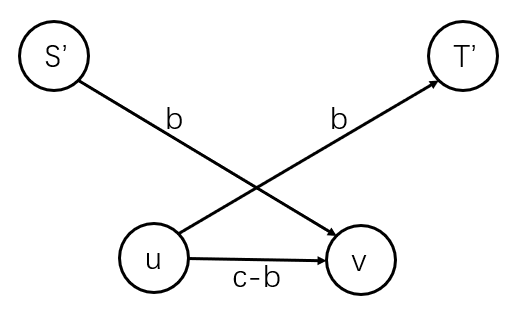
\includegraphics[scale = 0.5]{../src/graph/上下界网络流.png}

在新图跑一遍最大流之后检查一遍辅助边,如果有辅助边没满流则无解,否则把每条边的流量加上 $b$ 就是一组可行方案。

\paragraph{有源汇上下界最大流}
如果不需要判断是否有解的话,可以直接按照和上面一样的方法转化。因为附加边实际上算了两次流量,所以最终答案应该减掉所有下界之和。

(另外这里如果要压缩附加边的话,不能像无源汇的情况一样对每个点只开一个变量统计溢出的流量。正确的做法是进出流量各统计一下,每个点连两条附加边。)

如果需要判有解的话会出一点问题。这时候就需要转化成无源汇的情况,验证有解之后撤掉 $T$ 到 $S$ 的那条附加边,再从 $S$ 到 $T$ 跑一遍最大流。

\inputminted{cpp}{../src/graph/有源汇上下界最大流.cpp}

\paragraph{有源汇上下界最小流}
按照上面的方法转换后先跑一遍最大流,然后撤掉超级源汇和附加边,反过来跑一次最大流退流,最大流减去退掉的流量就是最小流。

\subsubsection{常见建图方法}

\begin{itemize}

\item \textbf{最大流/费用流}

流量不是很多的时候可以理解成很多条路径,并且每条边可以经过的次数有限。

\item \textbf{最小割}

常用的模型是 \textbf{最大权闭合子图}。当然它并不是万能的,因为限制条件可以带权值。

\begin{enumerate}

\item 如果某些点全部在 $S$ 集或者 $T$ 集,则获得一个正的收益

把这个条件建成一个点,向要求的点连 $+\infty$ 边,然后 $s$ 向它连 $+\infty$ 边。(如果是 $T$ 集就都反过来)

那么如果它在 $S$ 集,就一定满足它要求的点都在 $S$ 集,反之如果是 $T$ 集亦然。

\item 如果两个点不在同一集合中,则需要付出代价

建双向边,那显然如果它们不在同一集合中就需要割掉中间的边,付出对应的代价。

\item 二分图,如果相邻的两个点在同一集合则需要付出代价

染色后给一半的点反转源汇,就转换成上面的问题了。

\end{enumerate}

\end{itemize}

\subsubsection{例题}

\begin{itemize}

% \item 最大流



% \item 最小割

% \begin{enumerate}

% \item 切糕

% \end{enumerate}

\item 费用流

\begin{enumerate}

\item 序列上选总和尽量大的数,但连续 $k$ 个数中最多选 $p$ 个

费用流建图,先建一条 $n+1$ 个点的无限容量的链表示不选,然后每个 $i$ 向 $(i + k)$ 连边费用是第 $i$ 个位置的权值。答案是流量为 $p$ 的最大费用流,因为条件等价于选 $p$ 次并且每次选的所有数间隔都至少是 $k$。

\item 除此之外还要求连续 $k$ 个数中最少选 $q$ 个

任选一个位置把图前后切开,会发现通过截面的流量总和恰为 $p$。注意到如果走了最开始的链就代表不选,因此要限制至少有 $q$
的流量不走链,那么只需要把链的容量改成 $p - q$ 就行了。

\end{enumerate}

\end{itemize}

			
			\subsection{Stoer-Wagner全局最小割}
				\inputminted{cpp}{../src/graph/stoer-wagner.cpp}
			
		\section{数据结构}
			\subsection{历史和}

				EC-Final2020 G, 原题是询问某个区间有多少子区间, 满足子区间中数的种类数为奇数.

				离线之后转化成枚举右端点并用线段树维护左端点, 然后就是一个支持区间反转(0/1互换)和询问历史和的线段树.

				``既然标记会复合,就说明在两个标记中间没有经过任何 pushup 操作

				也就是说一个这两个标记对应着 相同的 0 的数量 以及 相同的 1 的数量

				那么标记对于答案的影响只能是 a * 0 + b * 1

				我们维护 a,b 即可''

				\inputminted{cpp}{../src/datastructure/ec20g.cpp}
			
			\subsection{二叉堆}
				\inputminted{cpp}{../src/datastructure/二叉堆.cpp}

		\section{字符串}
			\subsection{KMP}
				\inputminted{cpp}{../src/string/KMP.cpp}
				
				\subsubsection{ex-KMP}
					\inputminted{cpp}{../src/string/exKMP.cpp}
			\subsection[区间本质不同子串计数]{区间本质不同子串计数(后缀自动机+LCT+线段树)}
				\paragraph{问题} 给定一个字符串 $s$,多次询问 $[l, r]$ 区间的本质不同的子串个数,可能强制在线。

\paragraph{做法} 考虑建出后缀自动机,然后枚举右端点,用线段树维护每个左端点的答案。

显然只有 \texttt{right} 集合在 $[l, r]$ 中的串才有可能有贡献,所以我们可以只考虑每个串最大的 \texttt{right}。

每次右端点 + 1 时找到它对应的结点 $u$,则 $u$ 到根节点路径上的每个点,它的 \texttt{right} 集合都会被 $r$ 更新。

对于某个特定的左端点 $l$,我们需要保证本质不同的子串左端点不能越过它;因此对于一个结点 $p$,我们知道它对应的子串长度 $(val_{par_p}, val_p]$ 之后,在 $p$ 的 \texttt{right} 集合最大值减去对应长度,这样对应的 $l$ 内全部 + 1 即可。这样询问时就只需要查询 $r$ 对应的线段树中 $[l, r]$ 的区间和了。(当然旧的 \texttt{right} 对应的区间也要减掉)

实际上可以发现更新时都是把路径分成若干个整段更新 \texttt{right} 集合,因此可以用 LCT 维护这个过程。

时间复杂度 $O(n\log ^ 2 n)$,空间$O(n)$。当然如果强制在线的话,就把线段树改成主席树,空间复杂度就和时间复杂度同阶了。

\inputminted{cpp}{../src/string/samlct.cpp}

还有一份完整的代码,因为写起来确实细节挺多的。这份代码支持在尾部加一个字符或者询问区间有多少子串至少出现了 \textbf{两次},并且强制在线。

\inputminted{cpp}{../src/string/samlct2.cpp}


		\section{动态规划}
			
			\subsection{例题}
				\subsubsection{103388A Assigning Prizes 容斥}
	
	\paragraph{题意} 给定一个长为 $n$ 的序列 $a_i$,要求构造非严格递减序列 $b_i$,满足 $a_i \le b_i \le R$,求方案数。$n \le 5 \times 10 ^ 3, R, a_i \le 10 ^ 9$。
	
	\paragraph{做法} $a_i$ 的范围太大了,不能简单地记录上一位的值。

	考虑使用容斥。方便起见把 $a_i$ 直接变成 $R - a_i + 1$,条件就变成了 $b_i \le a_i$ 且 $b_i \ge b_{i - 1}$。

	这里有两个限制条件,可以固定 $b_i \le a_i$ 是必须满足的条件,只对 $b_i \ge b_{i - 1}$ 使用容斥,枚举哪些位置是比上一位小的(违反限制),其他位置随意。

	枚举后的形态一定是有若干个区间是严格递减的,其他位置随意。考虑如果一个区间 $[l, r]$ 是严格递减的,显然所有的数都 $< a_l$,所以这段区间的方案数就是 ${a_l \choose r - l + 1}$。另外实际上 $b_l$ 是没有违反限制的,所以这里对系数的贡献是 $(-1) ^ {r - l}$。

	考虑令 $dp_i$ 表示只考虑前 $i$ 个位置的答案,转移时自然就是枚举一个 $j$,然后计算 $dp_{j - 1}$ 乘上区间 $[j, i]$ 严格递减的方案数。另外还有一种情况是 $b_i$ 没有违反限制,这时显然直接在 $dp_{i - 1}$ 的基础上乘上一个 $a_i$ 就好了。(转移时还要注意,由于枚举的是严格递减区间,自然就不能枚举只有一个数的区间。

	\inputminted{cpp}{../src/dp/103388A.cpp}


		\section{计算几何}
			
			\subsection{最近点对}
				首先分治的做法是众所周知的。

有期望 $O(n)$ 的随机增量法:首先将所有点随机打乱,然后每次增加一个点,更新答案。

假设当前最近点对距离为 $s$,则把平面划分成 $s \times s$ 的方格,用哈希表存储每个方格有哪些点。

加入一个新点时,只需要枚举自身和周围共计 $9$ 个方格中的点,显然枚举到的点最多 $16$ 个。如果加入之后答案变小了,就 $O(n)$ 暴力重构。

前 $i$ 个点中 $i$ 是最近点对中的点的概率至多为 $\frac 2 i$,所以每个点的期望贡献都是 $O(1)$,总的复杂度就是期望$O(n)$。

如果对每个点都要求出距离最近的点的话,也有随机化的 $O(n)$ 做法:

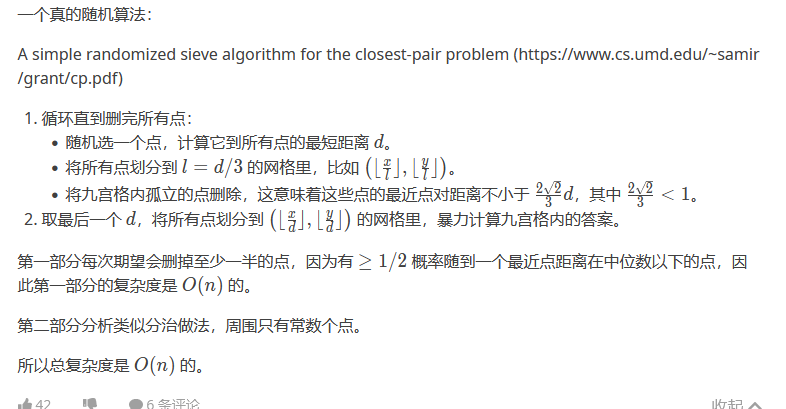
\includegraphics[width=0.8\linewidth]{../src/geometry/最近点对.png}


		\section{杂项}
			\subsection{STL}
				\subsubsection{vector}
	\begin{itemize}
		\item \mintinline{cpp}{vector(int nSize)}: 创建一个vector, 元素个数为nSize
		\item \mintinline{cpp}{vector(int nSize, const T &value)}: 创建一个vector, 元素个数为nSize, 且值均为value
		\item \mintinline{cpp}{vector(begin, end)}: 复制[begin, end)区间内另一个数组的元素到vector中
		\item \mintinline{cpp}{void assign(int n, const T &x)}: 设置向量中前n个元素的值为x
		\item \mintinline{cpp}{void assign(const_iterator first, const_iterator last)}: 向量中[first, last)中元素设置成当前向量元素
		\item \mintinline{cpp}{void emplace_back(Args&&... args)}: 自动构造并push\_back一个元素, 例如对一个存储pair的vector可以 \mintinline{cpp}{v.emplace_back(x, y)}
	\end{itemize}

\subsubsection{list}
	\begin{itemize}
		\item \mintinline{cpp}{assign()} 给list赋值 
		\item \mintinline{cpp}{back()} 返回最后一个元素 
		\item \mintinline{cpp}{begin()} 返回指向第一个元素的迭代器 
		\item \mintinline{cpp}{clear()} 删除所有元素 
		\item \mintinline{cpp}{empty()} 如果list是空的则返回true 
		\item \mintinline{cpp}{end()} 返回末尾的迭代器
		\item \mintinline{cpp}{erase()} 删除一个元素
		\item \mintinline{cpp}{front()} 返回第一个元素
		\item \mintinline{cpp}{insert()} 插入一个元素到list中
		\item \mintinline{cpp}{max_size()} 返回list能容纳的最大元素数量
		\item \mintinline{cpp}{merge()} 合并两个list
		\item \mintinline{cpp}{pop_back()} 删除最后一个元素
		\item \mintinline{cpp}{pop_front()} 删除第一个元素
		\item \mintinline{cpp}{push_back()} 在list的末尾添加一个元素
		\item \mintinline{cpp}{push_front()} 在list的头部添加一个元素
		\item \mintinline{cpp}{rbegin()} 返回指向第一个元素的逆向迭代器
		\item \mintinline{cpp}{remove()} 从list删除元素
		\item \mintinline{cpp}{remove_if()} 按指定条件删除元素
		\item \mintinline{cpp}{rend()} 指向list末尾的逆向迭代器
		\item \mintinline{cpp}{resize()} 改变list的大小
		\item \mintinline{cpp}{reverse()} 把list的元素倒转
		\item \mintinline{cpp}{size()} 返回list中的元素个数
		\item \mintinline{cpp}{sort()} 给list排序
		\item \mintinline{cpp}{splice()} 合并两个list
		\item \mintinline{cpp}{swap()} 交换两个list
		\item \mintinline{cpp}{unique()} 删除list中重复的元
	\end{itemize}

\subsubsection{unordered\_set/map}

\begin{itemize}
	\item \mintinline{cpp}{unordered_map<int, int, hash>}: 自定义哈希函数, 其中hash是一个带重载括号的类.
\end{itemize}

\subsubsection{自定义 Hash}
	\inputminted{cpp}{../src/misc/hash.cpp}
			
			\subsection{德州扑克}
				一般来说德扑里 Ace 都是最大的,所以把 Ace 的点数规定为 $14$ 会好写许多。

附一个高低奥马哈的参考代码,除了有四张底牌和需要比低之外和德扑区别不大。

\inputminted{cpp}{../src/misc/高低奥马哈.cpp}


	\end{multicols}

	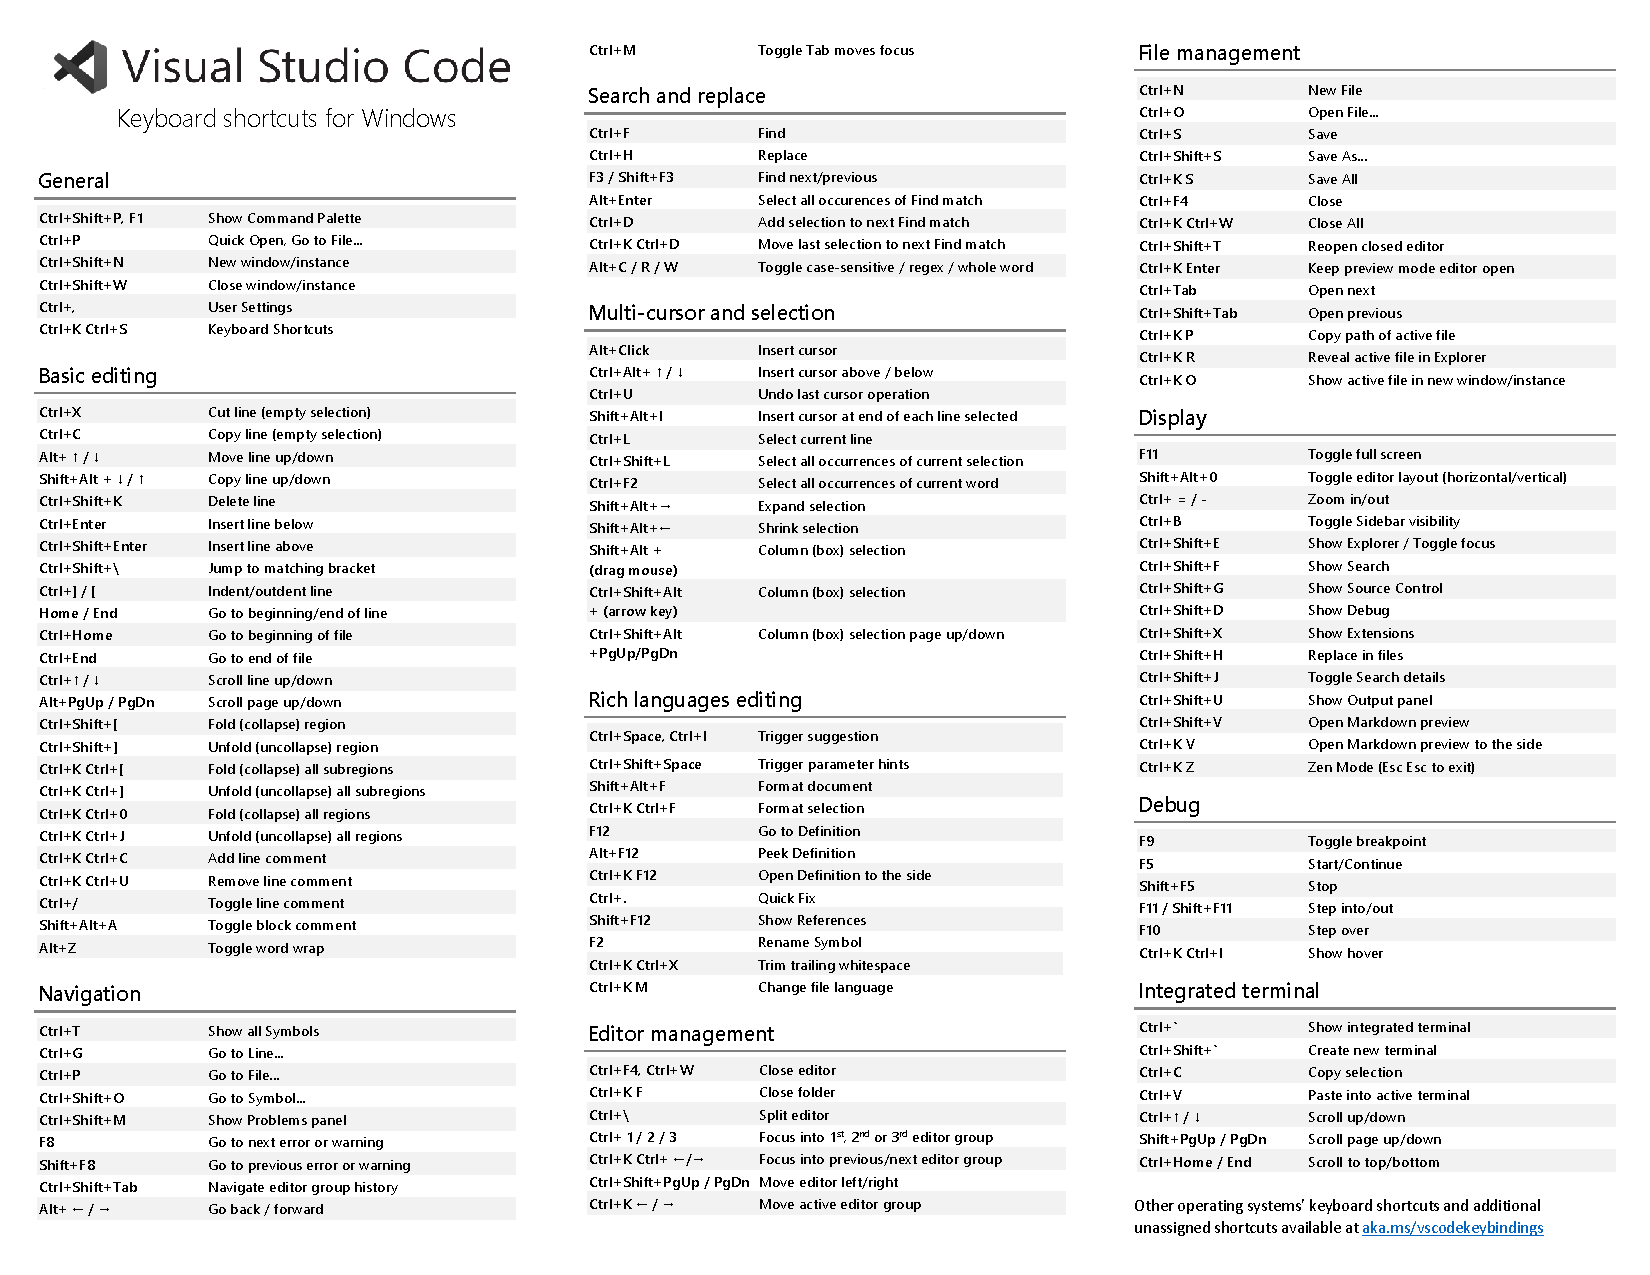
\includepdf[angle=270]{../src/misc/keyboard-shortcuts-windows.pdf}

	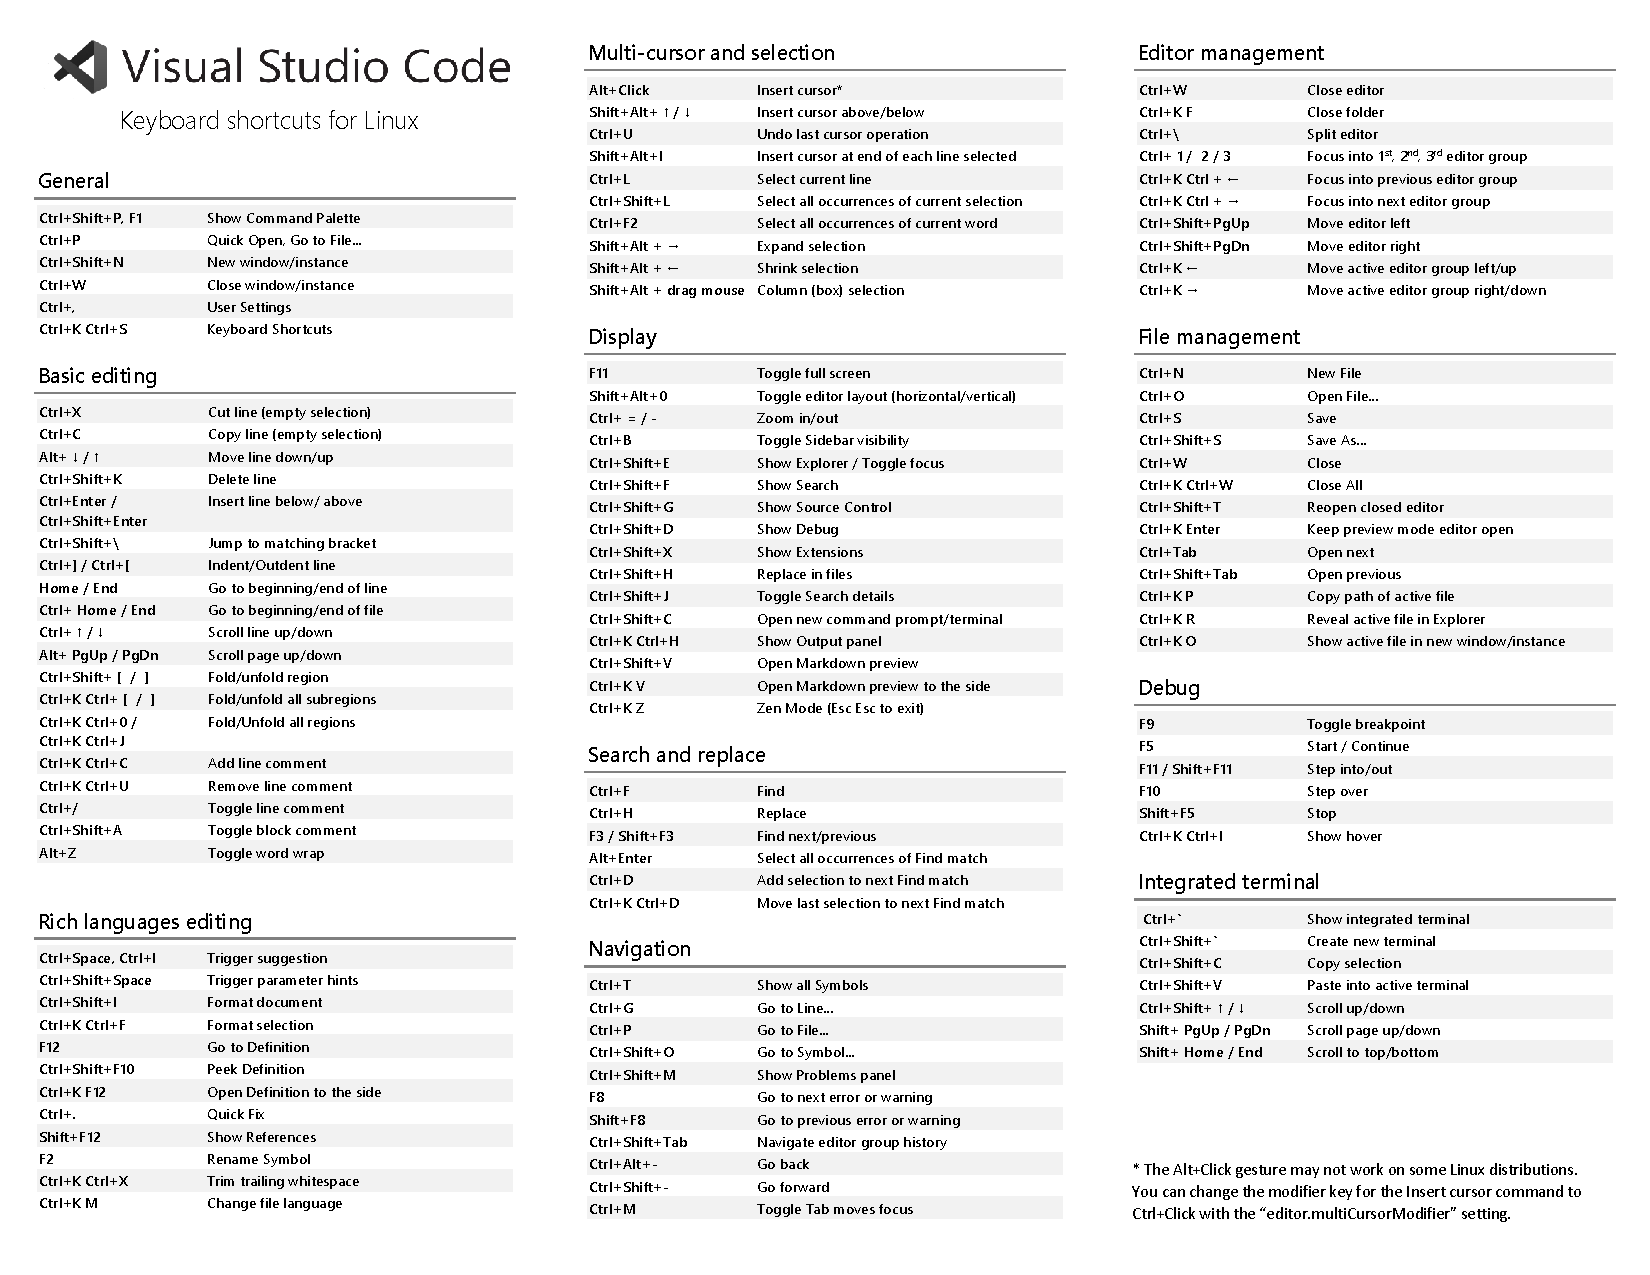
\includepdf[angle=270]{../src/misc/keyboard-shortcuts-linux.pdf}

	% \newpage
	% \ThisCenterWallPaper{1}{4.jpg}

	% \null
\end{document}